\documentclass[11pt]{article}
% Packages
\usepackage[utf8]{inputenc}
\usepackage[T1]{fontenc}
\usepackage[margin=1in]{geometry}
\usepackage{amsmath, amsthm, amsfonts, amssymb}
\usepackage{mathrsfs}           % \mathscr font.
\usepackage{setspace}
\usepackage[colorlinks=true,linkcolor=blue,citecolor=blue,urlcolor=blue,breaklinks]{hyperref}
\usepackage{graphicx}
\usepackage{booktabs}
\usepackage{xcolor}
\usepackage[style = authoryear, autocite=inline, doi=false,isbn=false,url=false]{biblatex}
\usepackage[sc]{titlesec} % make section headings \sffamily

% Header styling
% make headers \sffamily
\newpagestyle{main}[\sffamily]{
    \sethead{\thepage}{}{\sectiontitle}
    }
\pagestyle{main}
\usepackage{titling}
% make titling elements \sffamily
\pretitle{\begin{center}\sc \LARGE}
\preauthor{\begin{center}
            \large\sffamily \lineskip 0.5em%
            \begin{tabular}[t]{c}}
\predate{\begin{center}\sffamily\large}
\usepackage{abstract}
% make abstract title \sffamily
\renewcommand\abstractnamefont{\sffamily}
\titleformat{\section}[block]{\filcenter \Large \sc}{\thesection}{1em}{}
\usepackage{caption}
\captionsetup{font=sf, labelfont = bf}

% Define symbols and maths shortcuts
\DeclareRobustCommand{\bbone}{\text{\usefont{U}{bbold}{m}{n}1}}
\DeclareMathOperator{\EX}{\mathbb{E}} % expected value
\DeclareMathOperator{\V}{\mathbb{V}}
\DeclareMathOperator{\Prob}{\mathbb{P}}
\newcommand*{\trans}{^{\mathsf{T}}} %matrix transpose

\usepackage[long, nodayofweek]{datetime}
\usepackage[style = authoryear]{biblatex}

\addbibresource{../../literature/leapfrogging.bib}
\AtEveryBibitem{\clearfield{month}}
\newtheorem{assumption}{Assumption}
\usepackage{tikz}

\title{Party Competition between Regional Parties: Diverging from the Median}
\author{Tobias Nowacki\thanks{Stanford University, Calif., USA. \texttt{tnowacki@stanford.edu}. With thanks to David Laitin and Apoorva Lal. This proposal is for a joint project with Apoorva Lal in mind.}}

% Begin Document
\begin{document}

\maketitle

\onehalfspacing

\section{Introduction}

Blurb about what we want to do with this paper.
Another blurb about what this research proposal does.

\section{Literature}

Base this on ethnic outbidding; initial logic captured in Horowitz. Some studies show that ethnic outbidding does occur in European party systems. But so far no attempt to model the underlying mechanism. 

Ethnic outbidding model in \textcite{Chandra2005}: one centrist party (multiethnic coalition). Vulnerable to challengers from left/right. But if parties are office-seeking, it is not clear how a challenger to either side of the median can capture a larger vote-share... that is, the median position of the coalition should discourage challengers (unless they don't care about winning!)

This might be slightly different if we suddenly move from a two-party to a four-party world. That alone is a strong modelling assumption. But even then, the 'extreme' equilibrium only holds that the distribution of preferences is fully bipolar and there are no intermediate voters (this is crucial, acknowledged so much in fn. 12).

Instead, we show how we can get divergence towards the extremes when we have two different levels of elections, and two regional parties are in competition with one another.

Important question: polarisation driven by elite preferences or by voters?

\section{Theoretical framework: baseline}

National and regional distribution of preferences; parties are office-seeking. National party values national election more, regional parties only care about regional office.

The general framework of the model is as follows: let there be one national party, $N$, and either one or two regional parties, $R_1$ and $R_2$. There are two, separate elections: one for the regional legislature, and one for the national legislature. $N$ competes in the national and the regional elections, whereas $R_1, R_2$ only compete in the regional election. At first, let parties be office-oriented, that is, they set their policy such that they maximise their probability of winning. $N$ primarily cares about winning elections to the national legislature, and will prioritise winning these. (Further extensions of the model may weaken this assumption.)

Two crucial assumptions:
\begin{assumption}
    The national party runs in both the national and the regional election, but cares about winning office in the national election; the regional parties only run in the regional election and care about winning in it.
\end{assumption}
\begin{assumption}
    The national party can only set one policy position, $p_N$, with which it has to run in both elections.
\end{assumption}

(Justify Assumption 2).

Next, define the voter distribution for the two elections as follows: there is a continuuous, unidimensional policy space $P \in [0, 1]$. This policy space can represent the issue of regional autonomy (secession versus centralised government, for example), or how to split tax revenues between the national government and the regional government. It can also represent some other issue where preferences diverge heavily between the region and the rest of the country.

Let the distribution of voters in the national election be such that the median national voter is located at $\tilde{v}_N = 0.9$, that is, very close the 'unionist' pole of the policy dimension.\footnote{Not sure if a more specific functional form is necessary here -- national median is doing all the work in the model so far.} The distribution of voters in the regional election, for now, is a uniform distribution $\mathcal{F}_R \sim U[0, 1]$, such that $v_R = 0.5$.

Following the median voter theorem, parties competing in the national arena will thus have a strong incentive to place their policy position at this national median voter, such that $p_N = v_N = 0.9$.\footnote{Need to go into detail about one versus multiple national parties} By Assumption 2, they also have to take this position in the regional election, even though it may not be their best strategy. (However, since they primarily care about winning in the national election, $N$ will want to optimise for that)

Now, if the regional parties, $R_1, R_2$ competed for regional office in isolation, the median voter theorem would apply in the same sense, and both parties would locate themselves at $p_{R1} = p_{R2} = 0.5$. However, the existence of the national party, and its 'anchoring' at $0.9$, means that parties no longer converge at $0.5$. 

In the following subsections, I demonstrate how this leads to regional parties in competition with each other adopting policy positions to the left of the median voter (in equilibrium). This result may offer a first shot at a formal mechanism for elite-driven 'ethnic outbidding'.

\subsection{One regional party}

\begin{figure}[ht]
    \centering 
     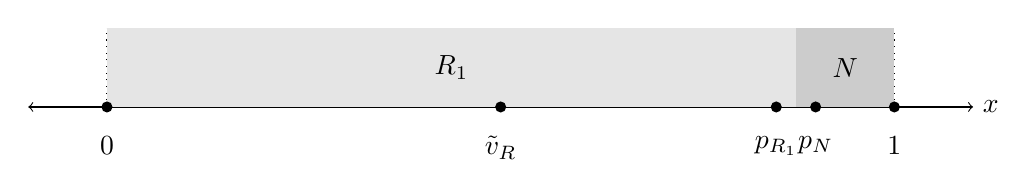
\begin{tikzpicture}
         % Axes
         \draw [<->] (-1,0) -- (11,0) node [right] {$x$};
         \draw [dotted] (0, 0) -- (0, 1);
         \draw [dotted] (10, 0) -- (10, 1);
         \draw [-] (0, 1) -- (10, 1);
         \fill [black!10] (0, 0) rectangle (8.75, 1);
         \draw (4.375, 0.5) node {$R_1$};
         \fill [black!20] (8.75, 0) rectangle (10, 1);
         \draw (9.375, 0.5) node {$N$};
         % Origin
         \node at (0,-.25) [below] {$0$};
         \node at (10, -.25) [below] {$1$};
         \node at (5, -.25) [below] {$\tilde{v}_R$};
         \node at (8.5, -.25) [below] {$p_{R_1}$};
         \node at (9, -.25) [below] {$p_{N}$};
         \coordinate (orig) at (0, 0);
         \coordinate (med)  at (5, 0);
         \coordinate (r1)   at (8.5, 0);
         \coordinate (N)    at (9, 0);
         \coordinate (end)  at (10, 0);
         \foreach \n in {orig, r1, med, N, end} \fill [black] (\n) circle (2pt);
     \end{tikzpicture}
     \caption{One national and one regional party; uniform distribution.} \label{fig:mod1}
 \end{figure}

 First, assume that there is only one regional party, $R_1$, that competes with $N$. 

 In equilibrium, it will position itself just to the left of $N$, and win the votes of everyone in the range from $[0, \frac{p_N + p_{R1}}{2}]$. $R_1$ has no incentive to move: moving further left would incur a vote loss towards $N$, and moving to the right of $N$ would leave them with a much smaller share of the distribution. Per assumption, $N$ cannot move its policy position. This is visualised in Figure \label{fig:mod1}. The resulting vote shares are $V_R = \frac{p_N + p_{R1}}{2}$ and $V_N = 1 - \frac{p_N + p_{R1}}{2}$.

As a consequence, the regional party positions itself close to the national party, and there is little issue competition on this dimension. Both are to the right of the regional median voter.\footnote{This is less problematic, because there is a reasonable argument that both the national and the regional party are close to the \textit{national} median voter. Whether that matters for evaluating the welfare outcome of this result for \textit{regional} elections is unclear.} It is likely that other divides (e.g., the classic left-right divide) are more salient in this scenario.

In practice, however, the regional party may position itself closer towards the median / the secessionist end, because of either inherent uncertainty or because of an intrinsic preference for a more autonomous policy. (see extensions to try and capture this. Another alternative is that they want to prevent any challengers from entering.) In either case, they will retain the majority of the vote share and thus capture office.\footnote{In the baseline model, the result suggests that they would be very close to $N$, purely because they'd rather win 90\% of the vote than `just' 60\%. That's not necessarily a plausible result, so the extensions may be crucial here.}

\subsection{Two regional parties}

\begin{figure}[ht]
    \centering 
     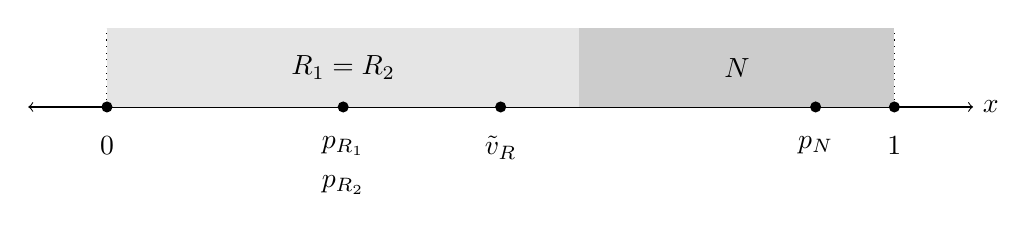
\begin{tikzpicture}
         % Axes
         \draw [<->] (-1,0) -- (11,0) node [right] {$x$};
         \draw [dotted] (0, 0) -- (0, 1);
         \draw [dotted] (10, 0) -- (10, 1);
         \draw [-] (0, 1) -- (10, 1);
         \fill [black!10] (0, 0) rectangle (6, 1);
         \draw (3, 0.5) node {$R_1 = R_2$};
         \fill [black!20] (6, 0) rectangle (10, 1);
         \draw (8, 0.5) node {$N$};
         % Origin
         \node at (0,-.25) [below] {$0$};
         \node at (5,-.25) [below] {$\tilde{v}_R$};
         \node at (10, -.25) [below] {$1$};
         \node at (3, -.25) [below] {$p_{R_1}$};
         \node at (3, -.75) [below] {$p_{R_2}$};
         \node at (9, -.25) [below] {$p_{N}$};
         \coordinate (orig) at (0, 0);
         \coordinate (med)  at (5, 0);
         \coordinate (r1)   at (3, 0);
         \coordinate (N)    at (9, 0);
         \coordinate (end)  at (10, 0);
         \foreach \n in {orig, r1, med, N, end} \fill [black] (\n) circle (2pt);
     \end{tikzpicture}
     \caption{One national and two regional parties; uniform distribution of voters.} \label{fig:mod1}
 \end{figure}

Next, suppose that there are two regional parties, $R_1$ and $R_2$ that compete together with $N$. I keep the assumption of uniformly distributed voters for now, before discussing a more general case in the next subsection.

As before, $N$ keeps its policy position fixed at $p_N = \tilde{v}_N$. In equilibrium, both regional parties position themselves at $p_N / 3$, such that they split the voters in the range $[0, 2 p_N/3]$ between them. Their vote shares are thus $V_{R1} = V_{R2} = p_N / 3$, whereas $N$ receives $V_N = 1 - \frac{2}{3} p_N$. Here, neither regional party has an incentive to move. Moving leftwards would only decrease their vote share to below $p_N / 3$; moving rightwards they would only swap votes they would gain from $N$ with those lost to the other regional party. The best they could do by moving rightwards is to position themselves at $2/3 p_N$, which would see them gain the same vote share again; however, in this case, $R_2$ could move closer again in order to optimise their vote share (thus, $(p_N / 3, 2 p_N/3, p_N) $ cannot be an equilibrium). Finally, there is no incentive to move to $p_N$: the split vote share with $N$ would be smaller than the split vote share with $R_2$. Note that this imposes the constraint $p_N \geq 0.75$ for this to be an equilibrium.\footnote{The vote share that $R$ gets in equilibrium must be greater than the vote share it would get if it were to share its policy position with $N$ instead, that is, the inequality $v_R \geq V_N / 2$ or $\frac{1}{3} p_N \geq (1 - \frac{2}{3} p_N) / 2$ must hold. This simplifies to $p_N \geq 0.75$.}

This result shows how the competition between the two regional parties can drive them to take on more extreme policy positions that are to the left of the regional median voter, and certainly far to the left of the national median voter. This captures a possible mechanism for `ethnic outbidding': given the fixed policy position of the national party, and their proximity to unionist-minded voters, the two regional parties compete for the attachment of the regional ethnicity instead, thus forgoing the compromise position between the two (i.e., the median voter).

\subsection{Two regional parties, polarised distribution}

The result from the previous subsection can be stated more generally, as long as the underlying distribution of voters is symmetric around the median voter, and the density is weakly increasing on either side of the median voter.\footnote{With `humps' in the distribution, the equilibrium may not work, as parties may take up more than 1/3 of the share if it's tightly clustered together} $\rightarrow$ conditions for symmetric polarisation!

Let $f(x)$ denote the pdf of voters with support over the policy dimension, $x \in [0, 1]$; let $F(x)$ denote the cdf, and $F^{-1}(x)$ the inverse of the cdf or the quantile function.

The previous equilibrium can then be restated in terms of parties' vote shares:

\begin{align*}
    p_{R1} = p_{R2} & = F^{-1}\Big(\frac{F(N)}{3}\Big) \\
    p_N & = \tilde{v}_N
\end{align*}

and the corresponding vote shares are:

\begin{align*}
    V_{R1} = V_{R2} & = \frac{1}{2} \int_{0}^{F^{-1}(\frac{2 F(N)}{3})} f(x) dx = \frac{1}{3} \int_{0}^{p_N} f(x) dx \\
    V_N & = 1 - \frac{2}{3} \int_{0}^{p_N} f(x) dx = \int_{\frac{p_N + p_R}{2}}^{1} f(x) dx
\end{align*}

(express this in terms of the cdf...)

As the distribution becomes more polarised, $p_R$ will be further removed from the regional median voter (why? -- discuss intuition).

One way to model a symmetric polarised distribution is the beta distribution. Figure X plots the distribution of voters, parties policy points in equilibrium, and their share of voters, for different parameters of the beta distribution. (This confirms the previous point.)

% In the more general case (weaker assumption: symmetric distribution), the position will be such that they locate their policy position at the first tercile of the voter mass with support $[0, p_N]$, such that:

% \begin{equation*}
%     F^{-1}(R_1, R_2) = F^{-1}\Big(\frac{F(N)}{3}\Big) 
% \end{equation*}

% and the resulting vote share for either $R_1, R_2$ is:

% \begin{equation*}
%     V_{R1} = V_{R2} = \frac{1}{2} \int_{0}^{F^{-1}(\frac{2 F(N)}{3})} f(x) dx 
% \end{equation*}


Main result: the more polarised the distribution becomes, the bigger is the deviation from the median.

\subsection{Results and Comparative Statics}

\begin{itemize}
    \item When polarisation increases, parties will take more extreme positions
    \item The more accommodating the national party is, the more extreme will the positions of the regional parties be.
\end{itemize}

\section{Theoretical framework: possible extensions}

\subsection{Policy-oriented parties}

\subsection{Uncertainty}

\subsection{Dynamic model}

\subsection{Coalition politics}

\section{Application (?)}

\section{Conclusion}


\renewcommand*{\mkbibnamefamily}[1]{\textsc{\textbf{#1}}}
\renewcommand*{\mkbibnamegiven}[1]{\textsc{#1}}
\printbibliography

\end{document}
